\chapter{Application Design}
\label{ch:Design}
Before making a start on of the implementation phase, a lot of effort was put into the creation of the application prototype. Prototyping is the process of developing the initial model of the future application in order to determine its correct structure, functionality and the general concept behind it. A prototype is just a model and may differ from the final product.

In order to fully describe a new product, the following aspects of its design should be modelled: product functionality, visual design and navigation. Those aspects are best covered by different techniques: user stories for the application functionality, activity diagrams to describe the user journeys and sketches to capture the visual design. The modelling process will be illustrated in detail in this chapter. 

First, the project requirements outlined in the previous chapter were used in order to create a mind map. This is needed for brainstorming and allows the setting out of the initial ideas about what the visual design and the user experience should be. The next step is to produce hand-drawn wireframes that were sketched for each individual page of the application. To complement the wireframes, a set of user journeys were developed to describe the user interaction with the system. 

In summary, this chapter describes the process of transforming project requirements into the system design. Several design elements (website structure mind map, a set of wireframes) were produced before the implementation phase. Other elements (user stories, activity diagrams and the database schema) were designed in iterations, alongside with the development of the high-level features introduced in the chapter "Requirements Analysis" \ref{ch:requirementanalysis}. During the prototyping phase the main focus was on creating a visually appealling, simple and highly usable design. 

\section{Application Structure}
\label{sec:applicationstructure_design}
The prototyping process started with producing a large mind map of the future application. The mindmapping is a very useful way to brainstorm on the initial ideas, capture and organise them and was an extremely beneficial tool for this project in particular. The final version of the diagram puts together the structure of application pages, navigation scenarios and other ideas relevant to the visual design. A part of the developed mind map can be found in the figure below.

\begin{figure}[H]
	\begin{center}
		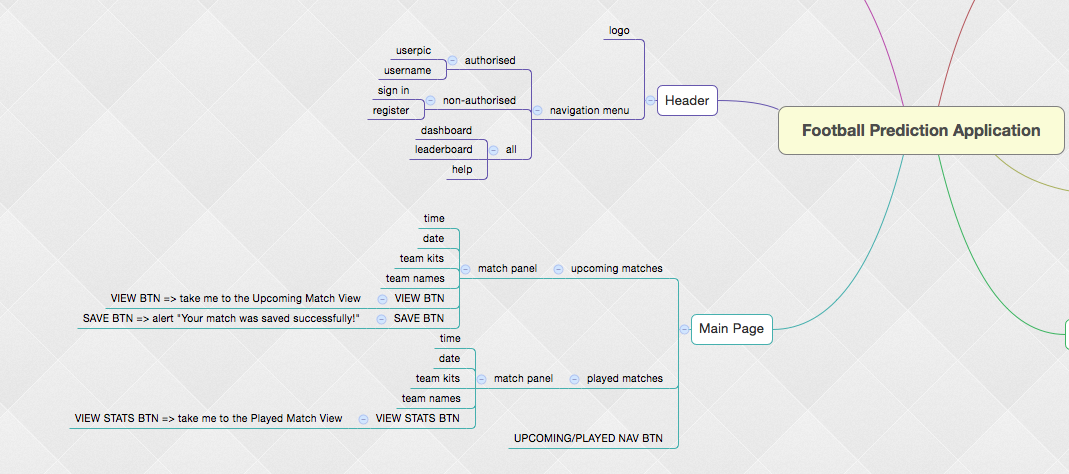
\includegraphics[width=.90\textwidth]{design/images/mindmap}
		\caption{Mind map capturing the results of initial brainstorming on the application structure and navigation scenarios.}
		\label{fig:using:mindmap}
	\end{center}
\end{figure}

\section{Branding and Visual Design}
\label{sec:visdesign_design}
At this stage of the prototyping process it was important to decide on a suitable name for the future application. Below is the list of some names that were considered.

\begin{itemize}
	\item Too Close To Call
	\item Sure Thing
	\item Footy Expert
	\item Beating the Odds
\end{itemize}

\emph{SureThing} was chosen as the project name for being unique, simple and catchy, whilst expressing the essence of the future application. The name evokes optimistic feelings and is quite suitable for a prediction system that is transparent to its users and will increase their chances to win a bet in the long run. 

As it can be seen from the long list of mandatory requirements, the project will require a lot of time to be invested in implementing its functionality. Therefore, it was decided to make use of the Twitter Bootstrap framework on the front end \citep{documentation:Bootstrap3} \citep{web:templateProgressus} in order to reduce the amount of time spent developing the visual side of the application and create simple and consistent interface. As a result, the final design is a mixture of ready-made solutions and my own ideas on how to visualise unique elements of the application layout, such as dashboard side menu, match panels in matches overview, the layout for the prediction modules in upcoming match view, etc. 

\section{Analysis of the competitors experience}
\label{sec:competitors_prototype}
As the next step, I took another look at the existing websites, expecting to get some ideas on how to approach the visual side of the website and to improve its usability. This step is an important stage of an application prototyping process: it allows to learn from the best design practices and possibly avoid potential errors. The usual practice is to concentrate on few websites of the direct competition as a first step. However, it was not possible to identify the direct competitors, as the idea behind the project is quite unique. Therefore, I analysed several football statistics and community websites, namely \emph{WhoScored?} \citep{source:whoscored}, \emph{Goal.com} \citep{source:goal} and \emph{OLGB Betting Community} \citep{source:olgb}, making a note of how those websites present football statistics to their users, what are the main differences between the presentation of an unplayed and played match and what interesting features each website offers to its audience. This analysis served as a great source of inspiration and the basis for the next step - producing the hand-drawn wireframes.

\section{Wireframes}
\label{sec:wireframes_design}
In the early stages of prototyping, a piece of paper and a pencil are the first choice of many designers. Sketching has a number of advantages when compared to the use of the graphic design software, such as Fireworks or Photoshop. With the editors it is easy to get distracted by brushing up unnecessary details too early. On the opposite side, sketches allow the quick expression of ideas and offer a lot of flexibility. It is easy to add notes, make small changes or replace an outdated sketch with a fresh one.

In this project, each of the sketches represented a separate “view” of the website. The scale of a “view” might differ. For example, some sketches show a whole page (home page, dashboard page, etc.), others only capture an important part of a page in more detail.  Below can be found scans of some of the paper wireframes used for this project.

\begin{figure}[H]
	\begin{center}
		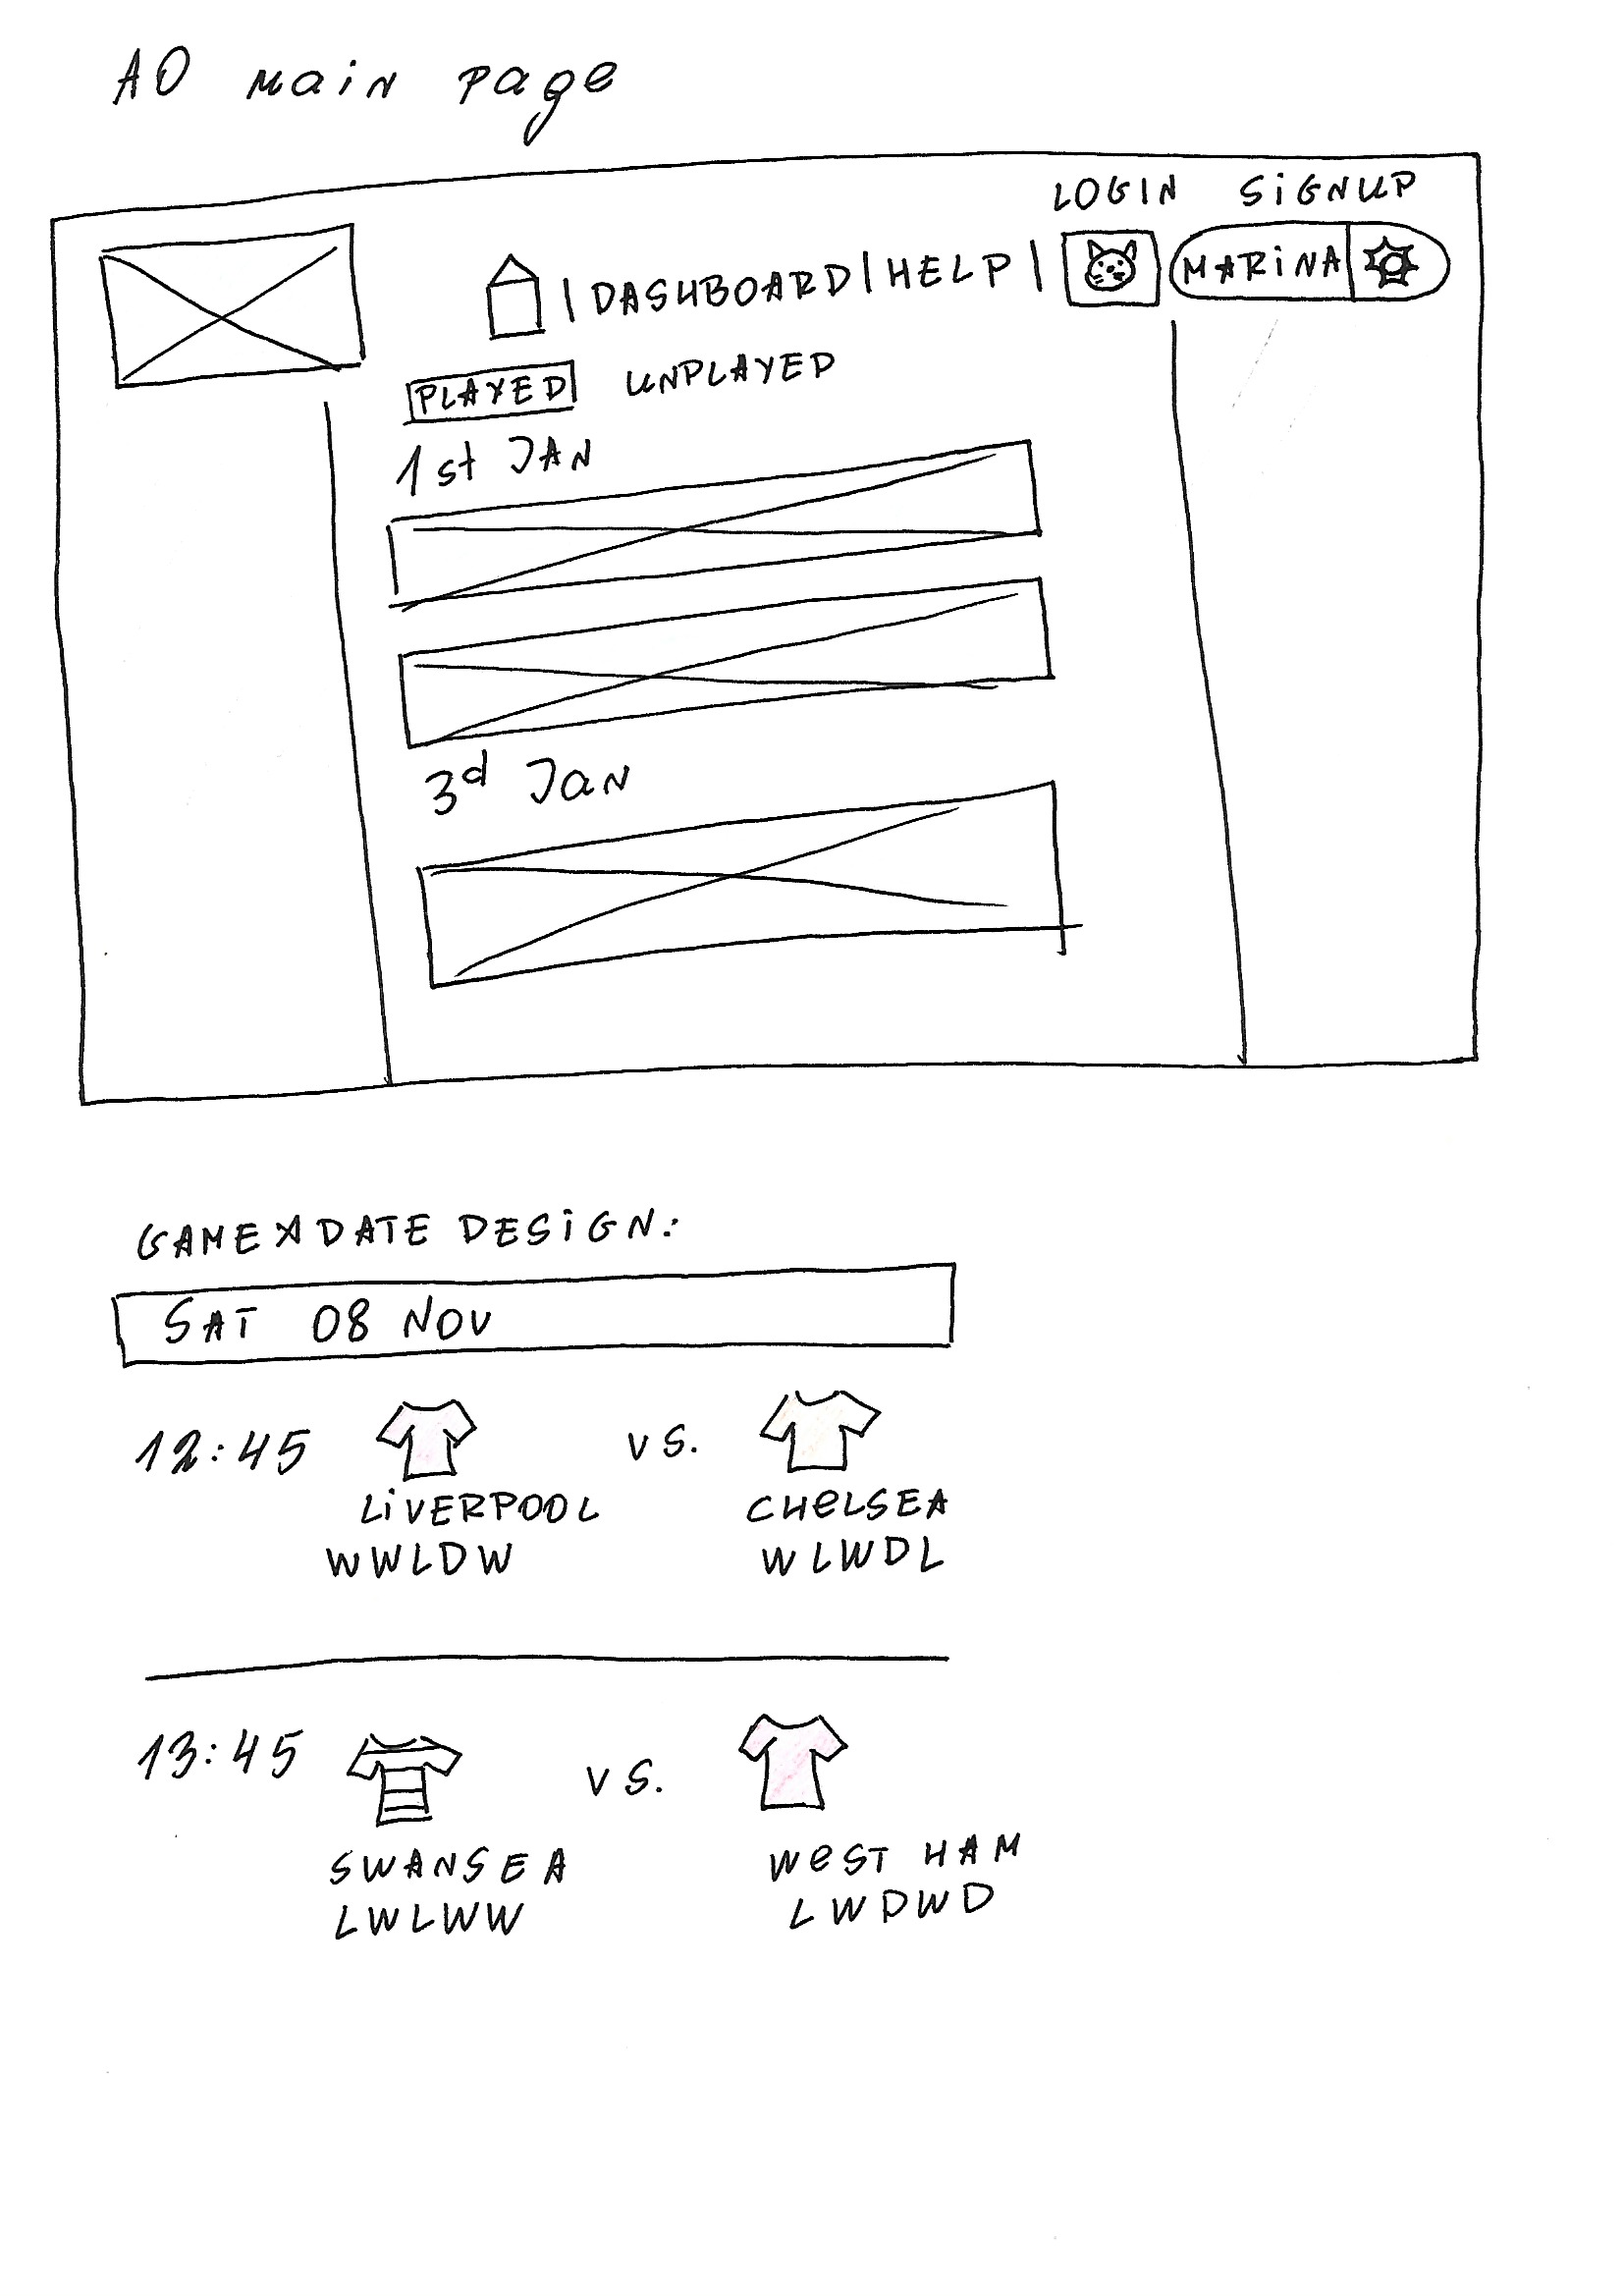
\includegraphics[width=.90\textwidth]{design/images/A0.jpg}
		\caption{A wireframe of the main page of the website.} \label{fig:using:wireframe_a0}
	\end{center}
\end{figure}

\begin{figure}[H]
	\begin{center}
		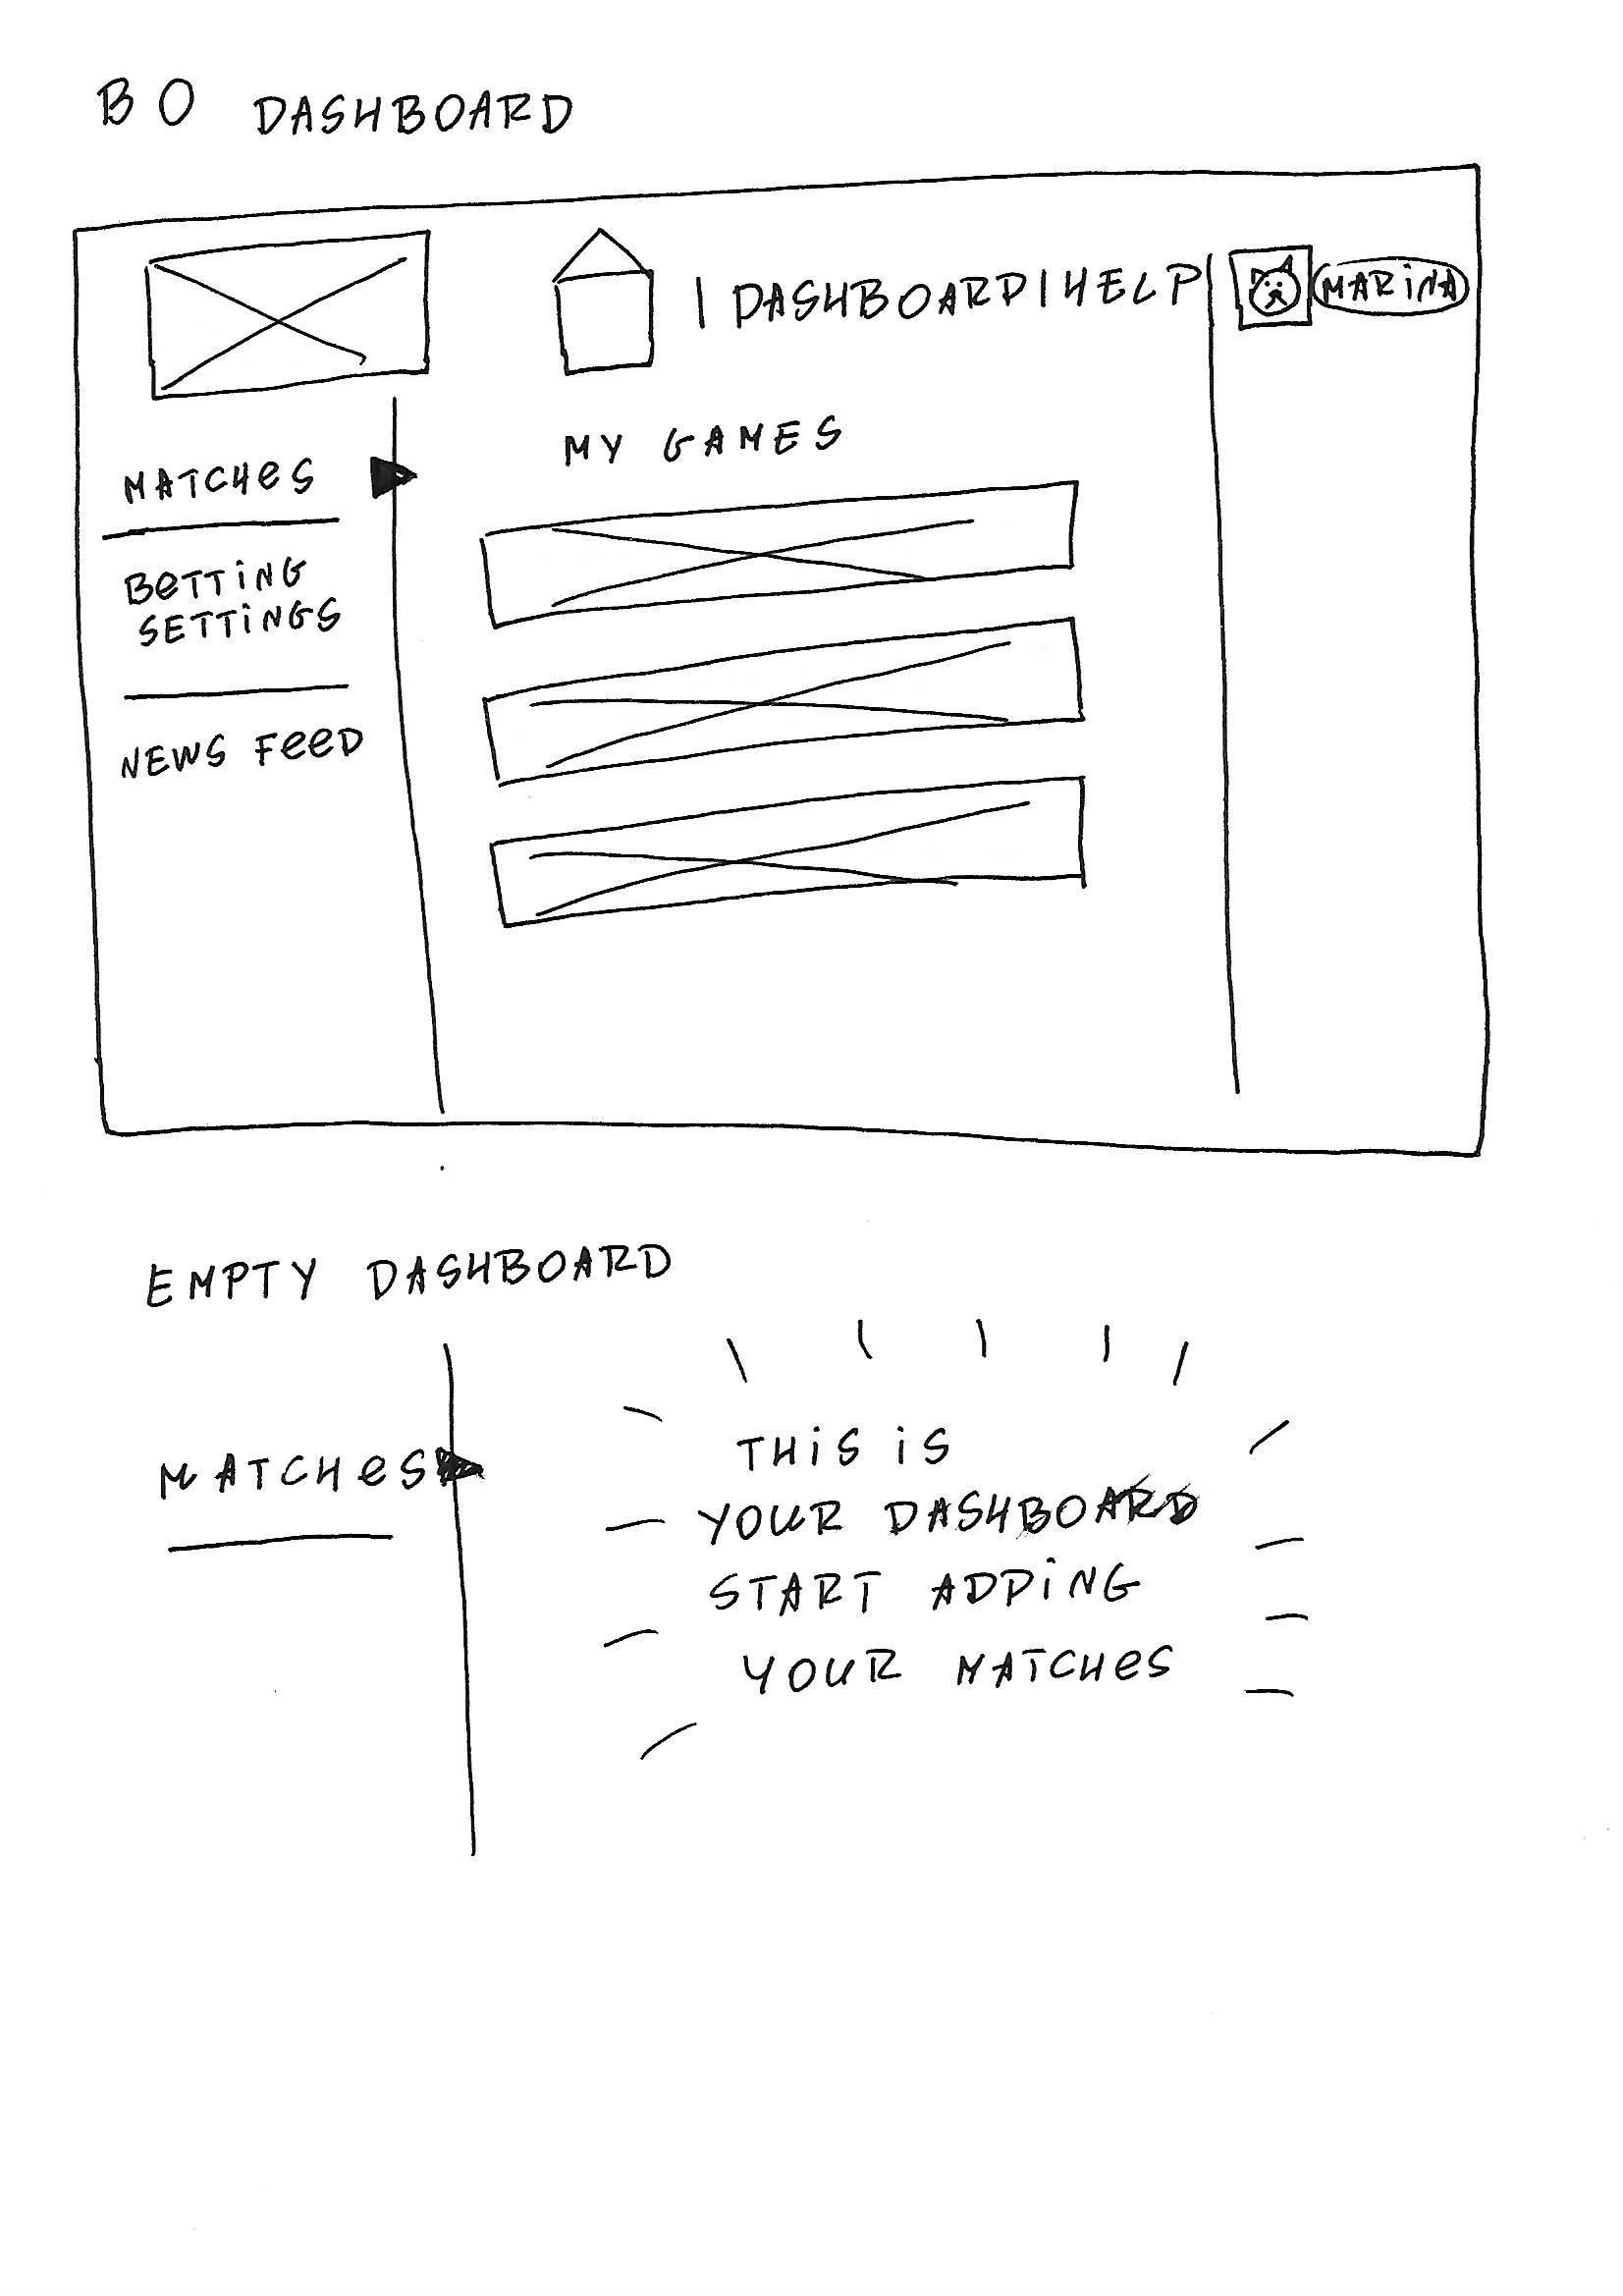
\includegraphics[width=.90\textwidth]{design/images/B0.jpg}
		\caption{A wireframe of the dashboard of the website, displaying the overview of the saved matches.} \label{fig:using:wireframe_b0}
	\end{center}
\end{figure}

\begin{figure}[H]
	\begin{center}
		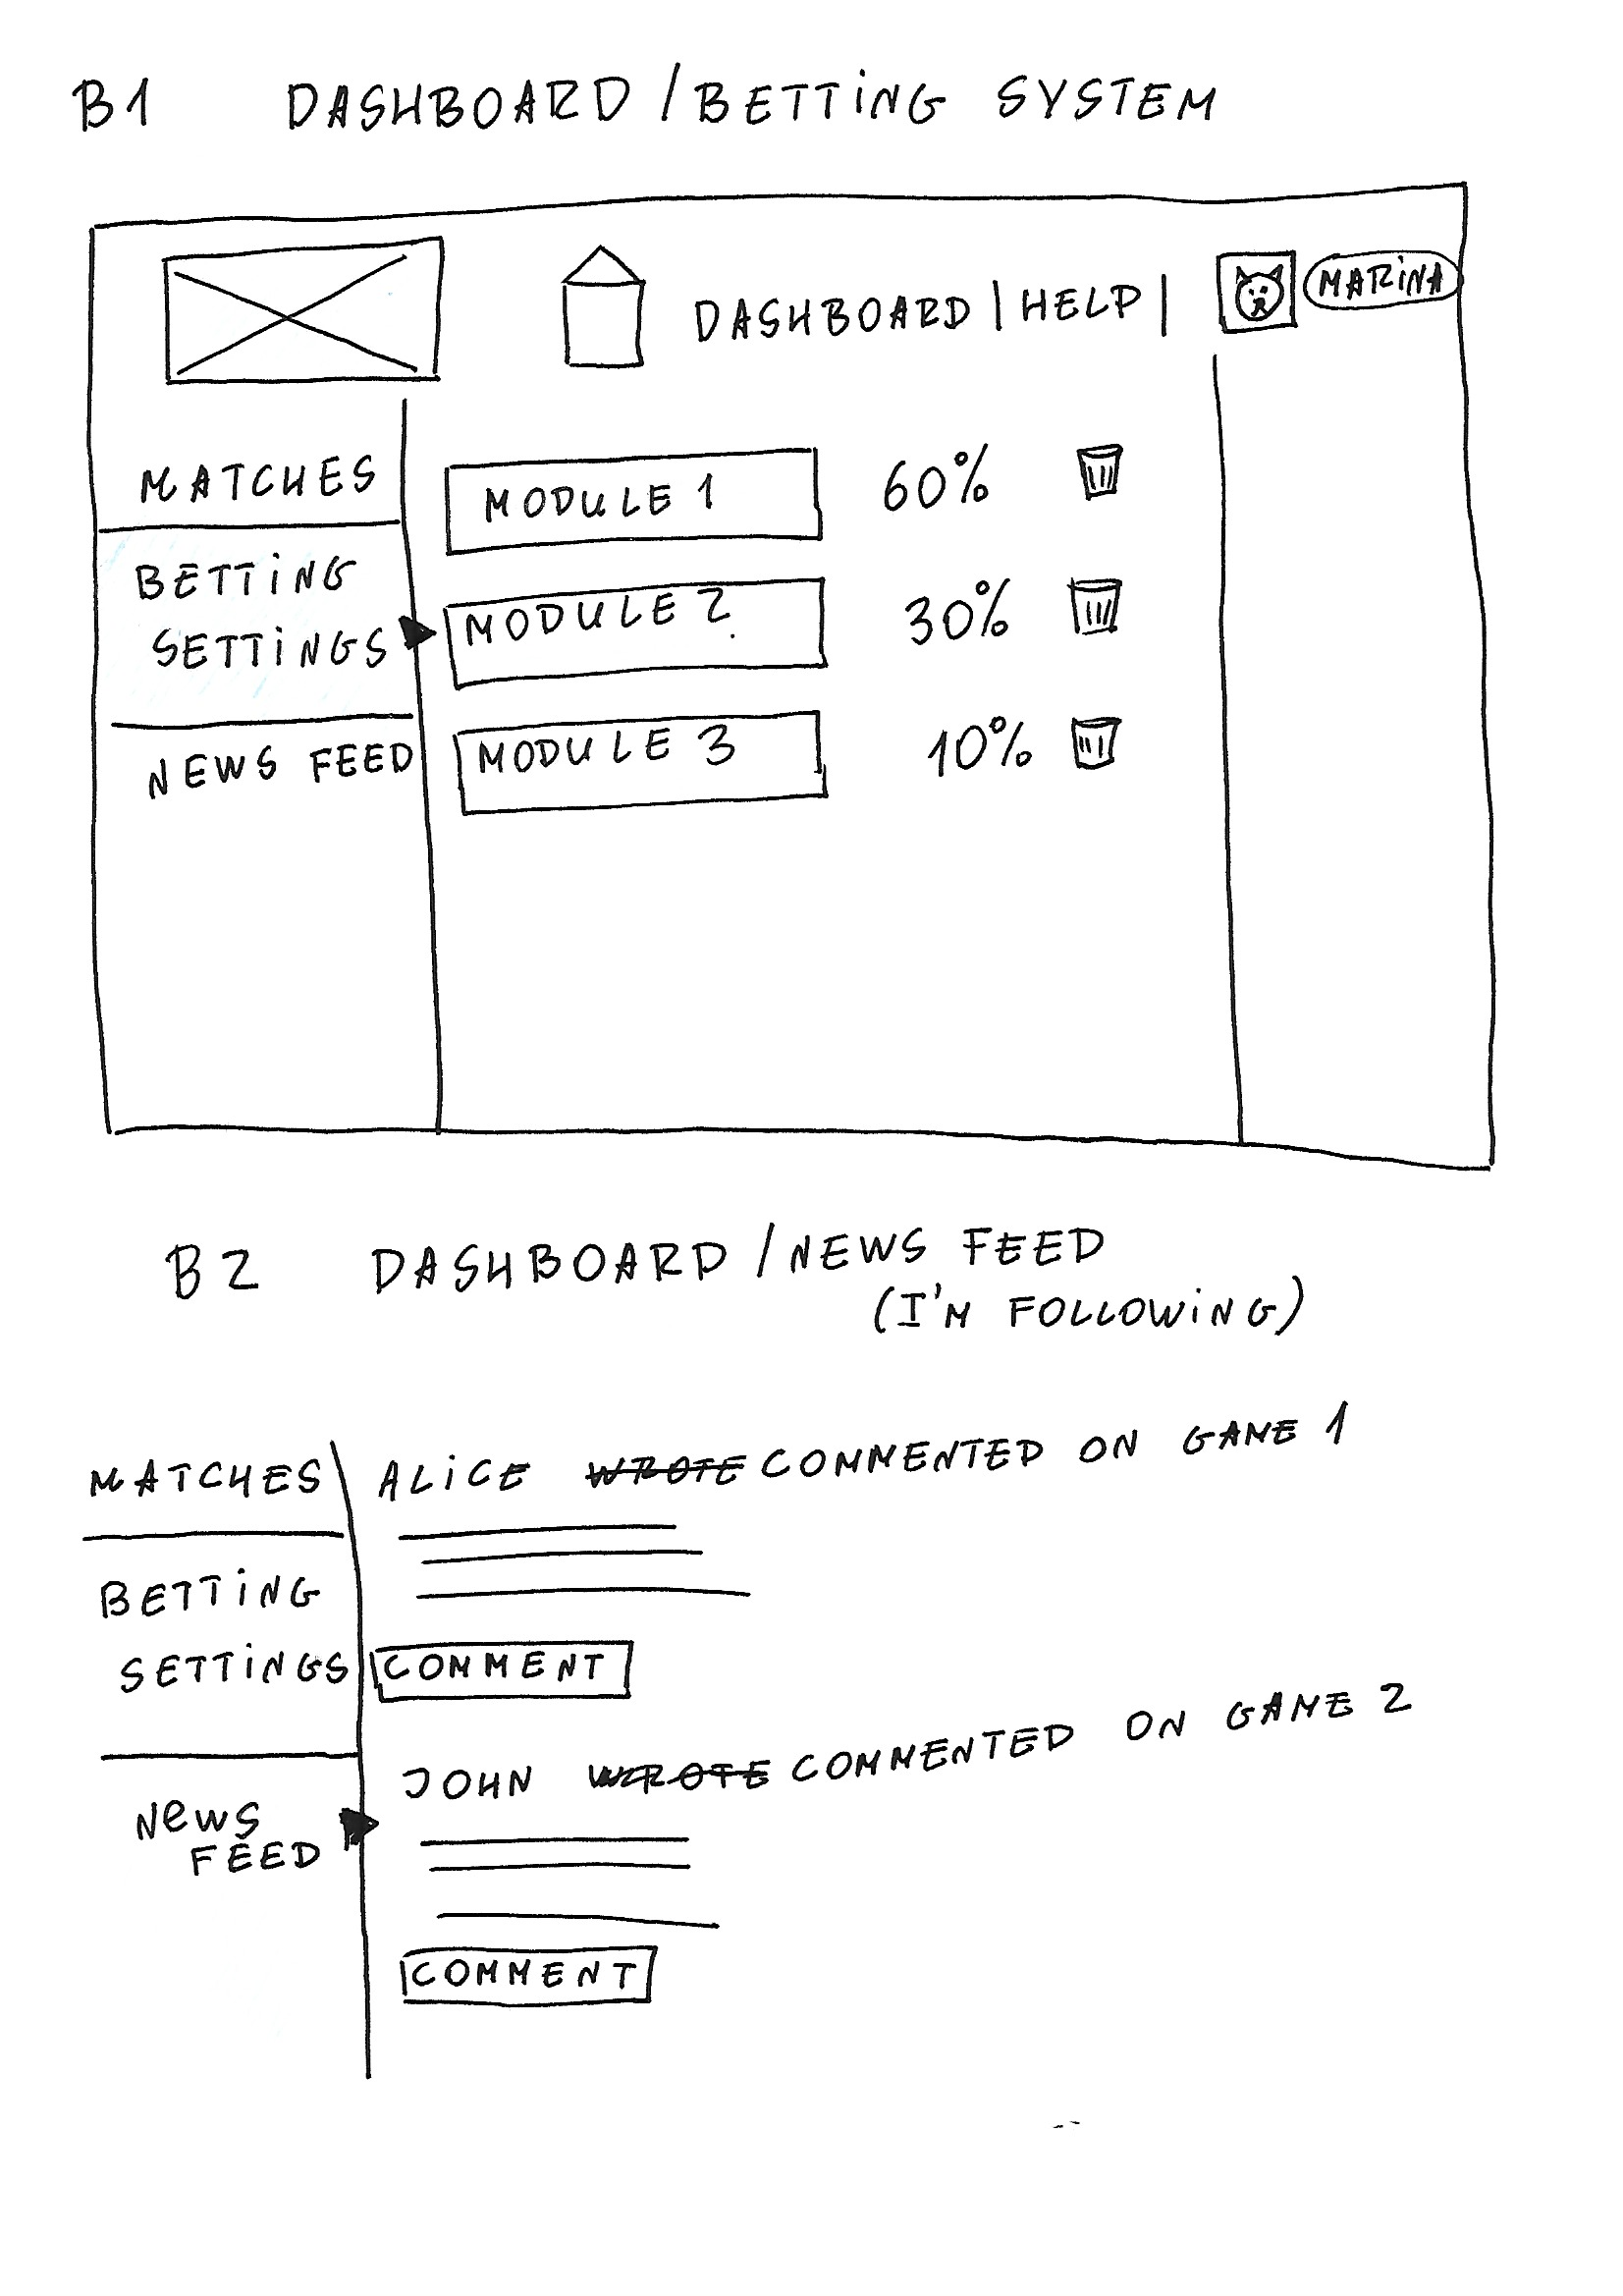
\includegraphics[width=.90\textwidth]{design/images/B1.jpg}
		\caption{A wireframe of the dashboard of the website, displaying the prediction settings form.} \label{fig:using:wireframe_b1}
	\end{center}
\end{figure}

\begin{figure}[H]
	\begin{center}
		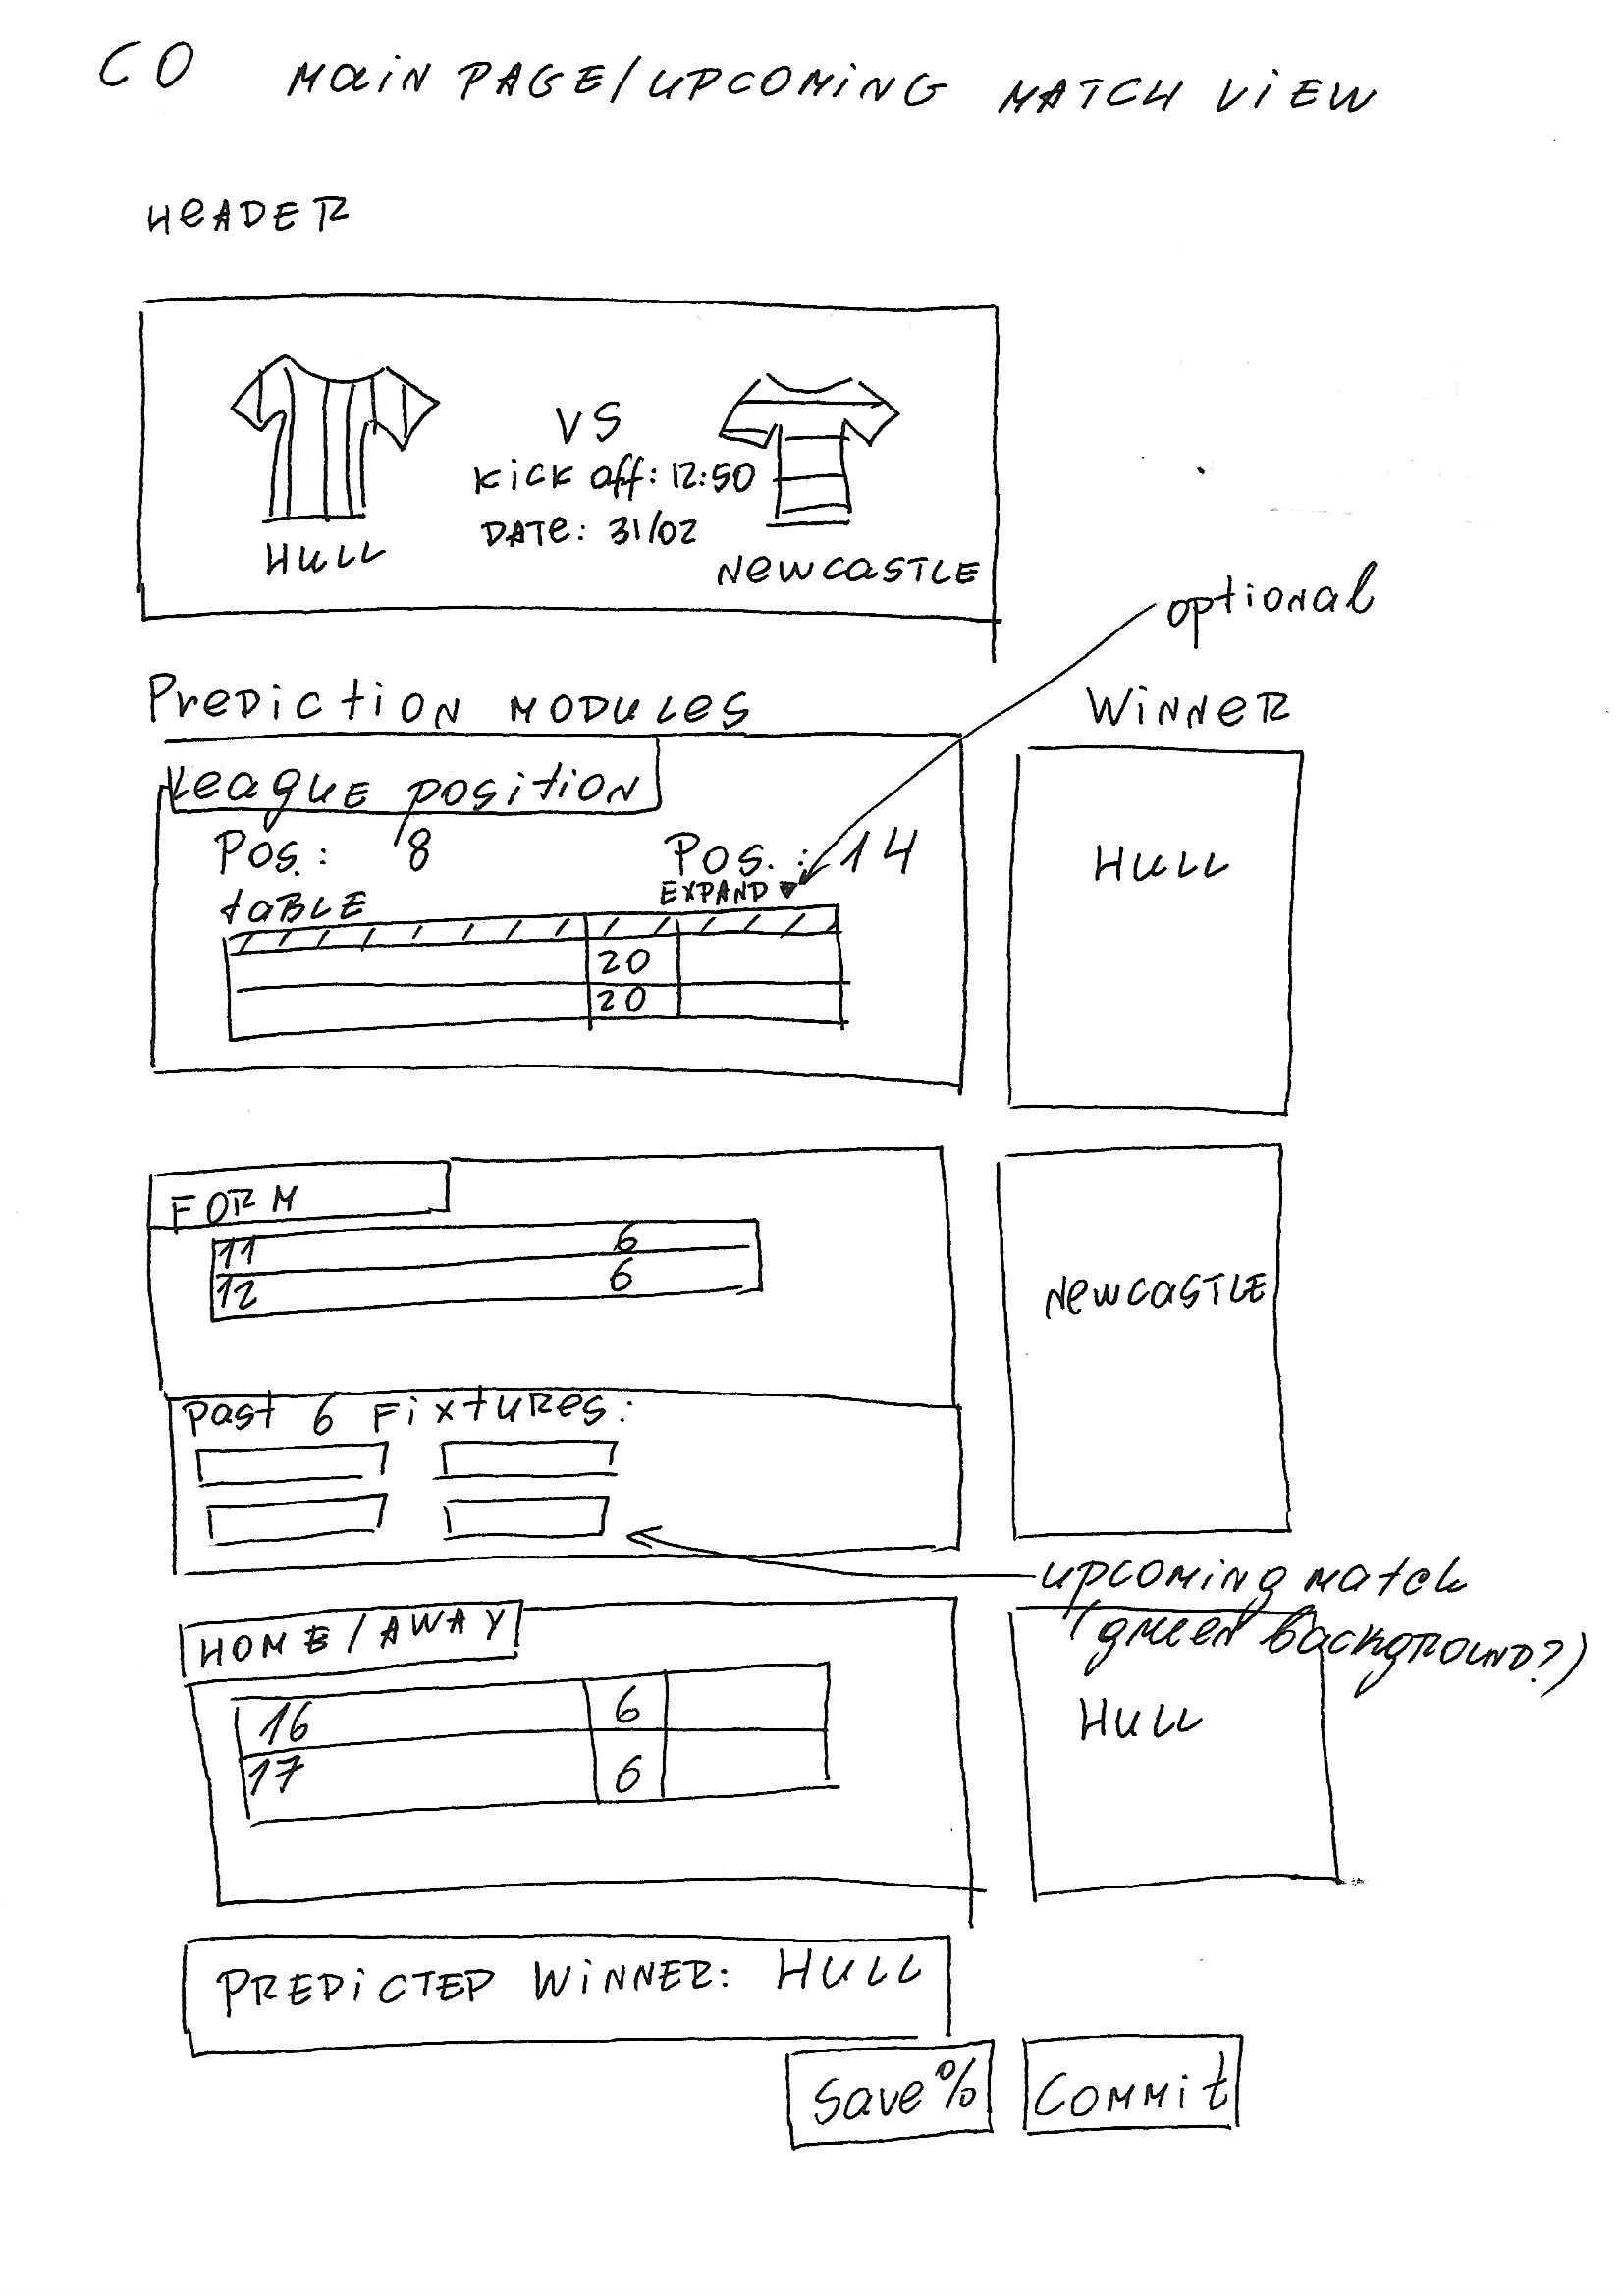
\includegraphics[width=.90\textwidth]{design/images/C0.jpg}
		\caption{A wireframe displaying an example of an upcoming match.} \label{fig:using:wireframe_c0}
	\end{center}
\end{figure}

\begin{figure}[H]
	\begin{center}
		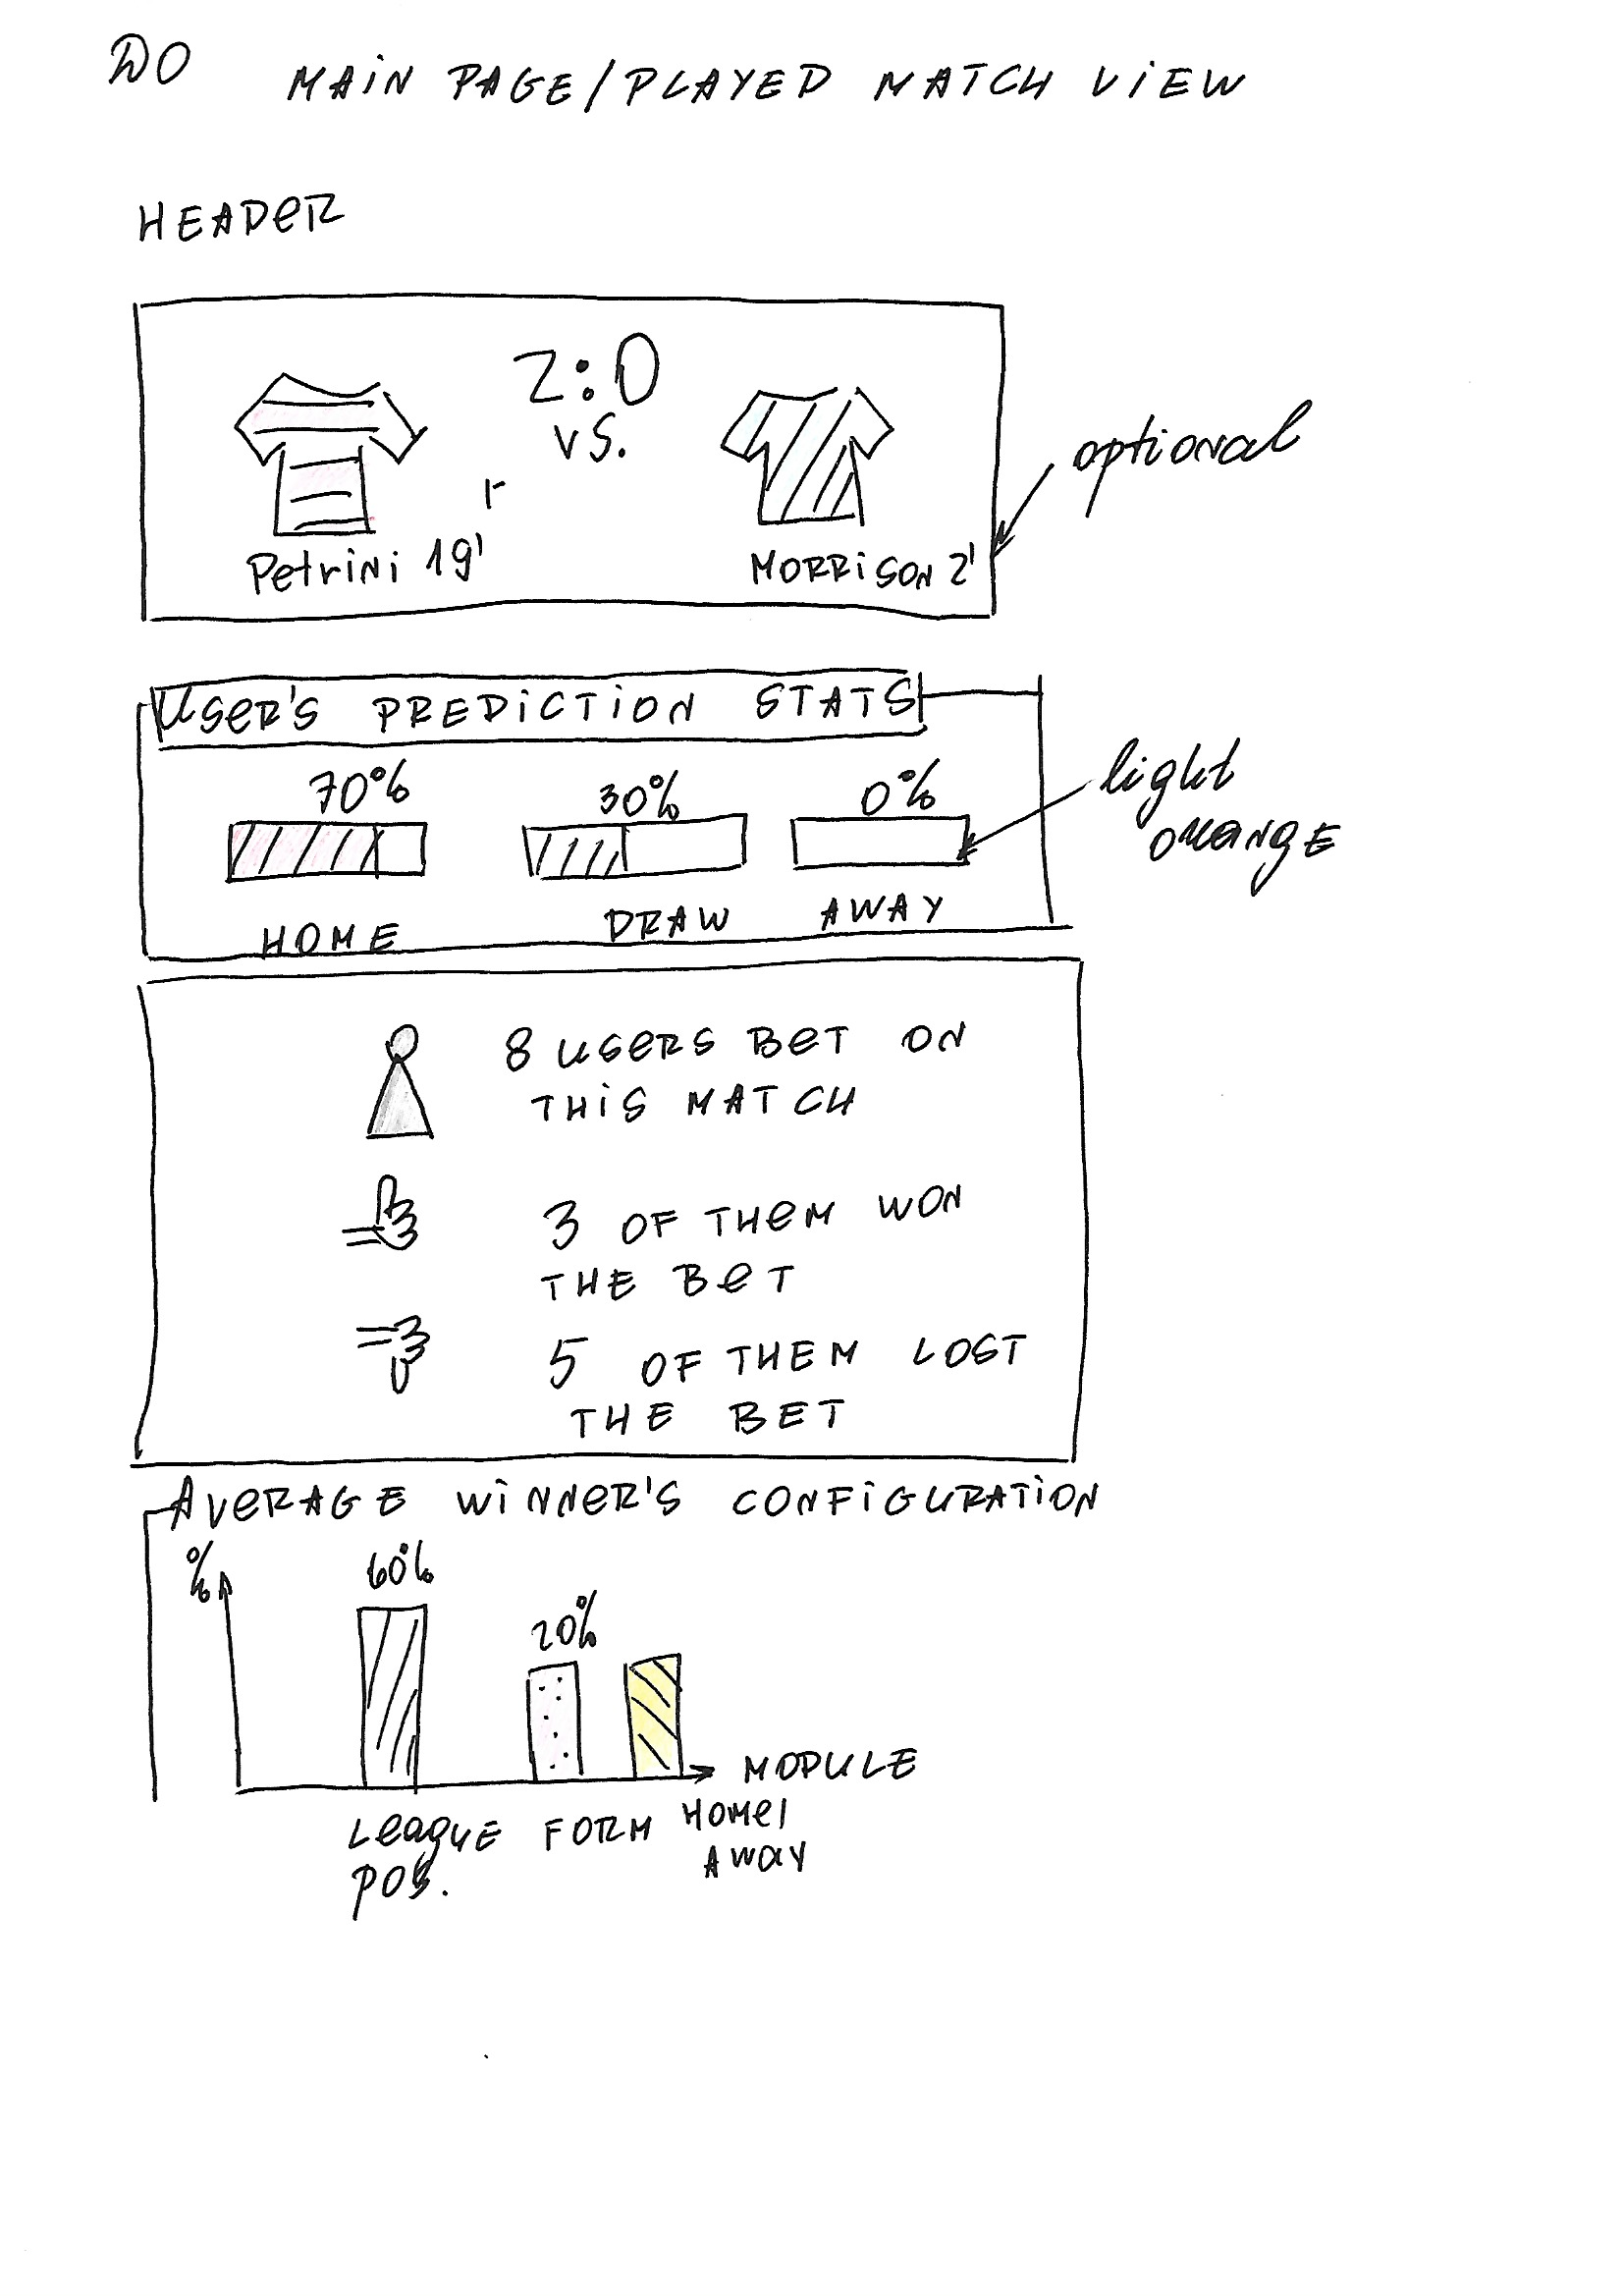
\includegraphics[width=.90\textwidth]{design/images/D0.jpg}
		\caption{A wireframe displaying the stats of a played match.} \label{fig:using:wireframe_d0}
	\end{center}
\end{figure}

\section{User Stories}
\label{userstories_design}
To describe the application functionality, a set of user stories was produced. User stories serve the similar purpose as the more traditional use cases, but they are not exactly the same. A use case is a graphical description of the interaction between the user and the system. On the other hand, a user story is usually a short sentence that expresses the need for product functionality from a user point of view. User stories are a more lightweight, informal version of the use cases. They are also another way to present the project requirements.

\begin{itemize}
	\item  As an Anonymous User, I would like to register with the application so I can use its full functionality.
	\item As an Application User, I would like to edit the information associated with my profile.
	\item As an Application User,  I want to be able to browse through the matches list and save a couple of them to my dashboard so I can review them later. 
	\item As an Application User, I would like to make a bet on a particular match.
	\item As an Application User, I want to see other players' performance so I can compare my performance to others. 
	\item As an Application User, I want to update my prediction settings so I can improve my betting system and a probability of winning. 
\end{itemize}

\section{Activity Diagrams}
\label{activitydiagrams_design}
In order to illustrate user interaction with the system and to complement the user stories, a number of activity diagrams were created. The diagrams can be very useful in terms of visualising the workflow and linking together individual user stories.  

\begin{figure}[H]
	\begin{center}
		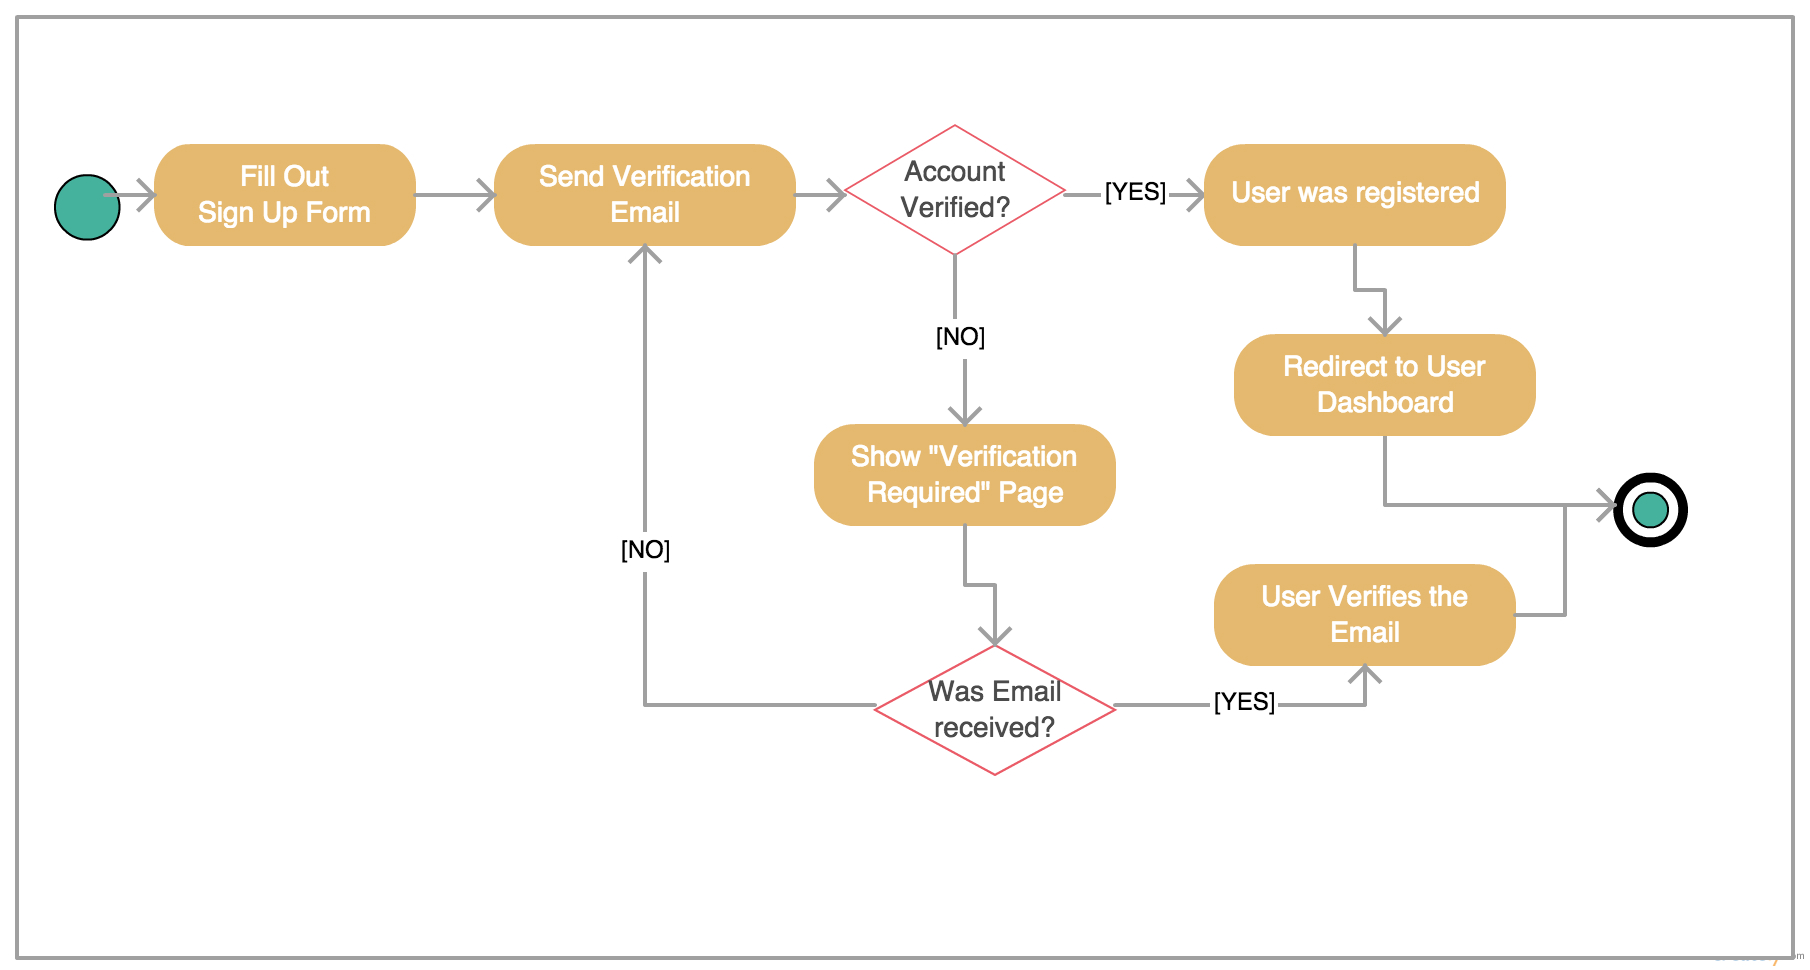
\includegraphics[width=.90\textwidth]{design/images/ad_1.jpg}
		\caption{User Sign Up activity diagram.} \label{fig:using:activitydiagram1}
	\end{center}
\end{figure}

\begin{figure}[H]
	\begin{center}
		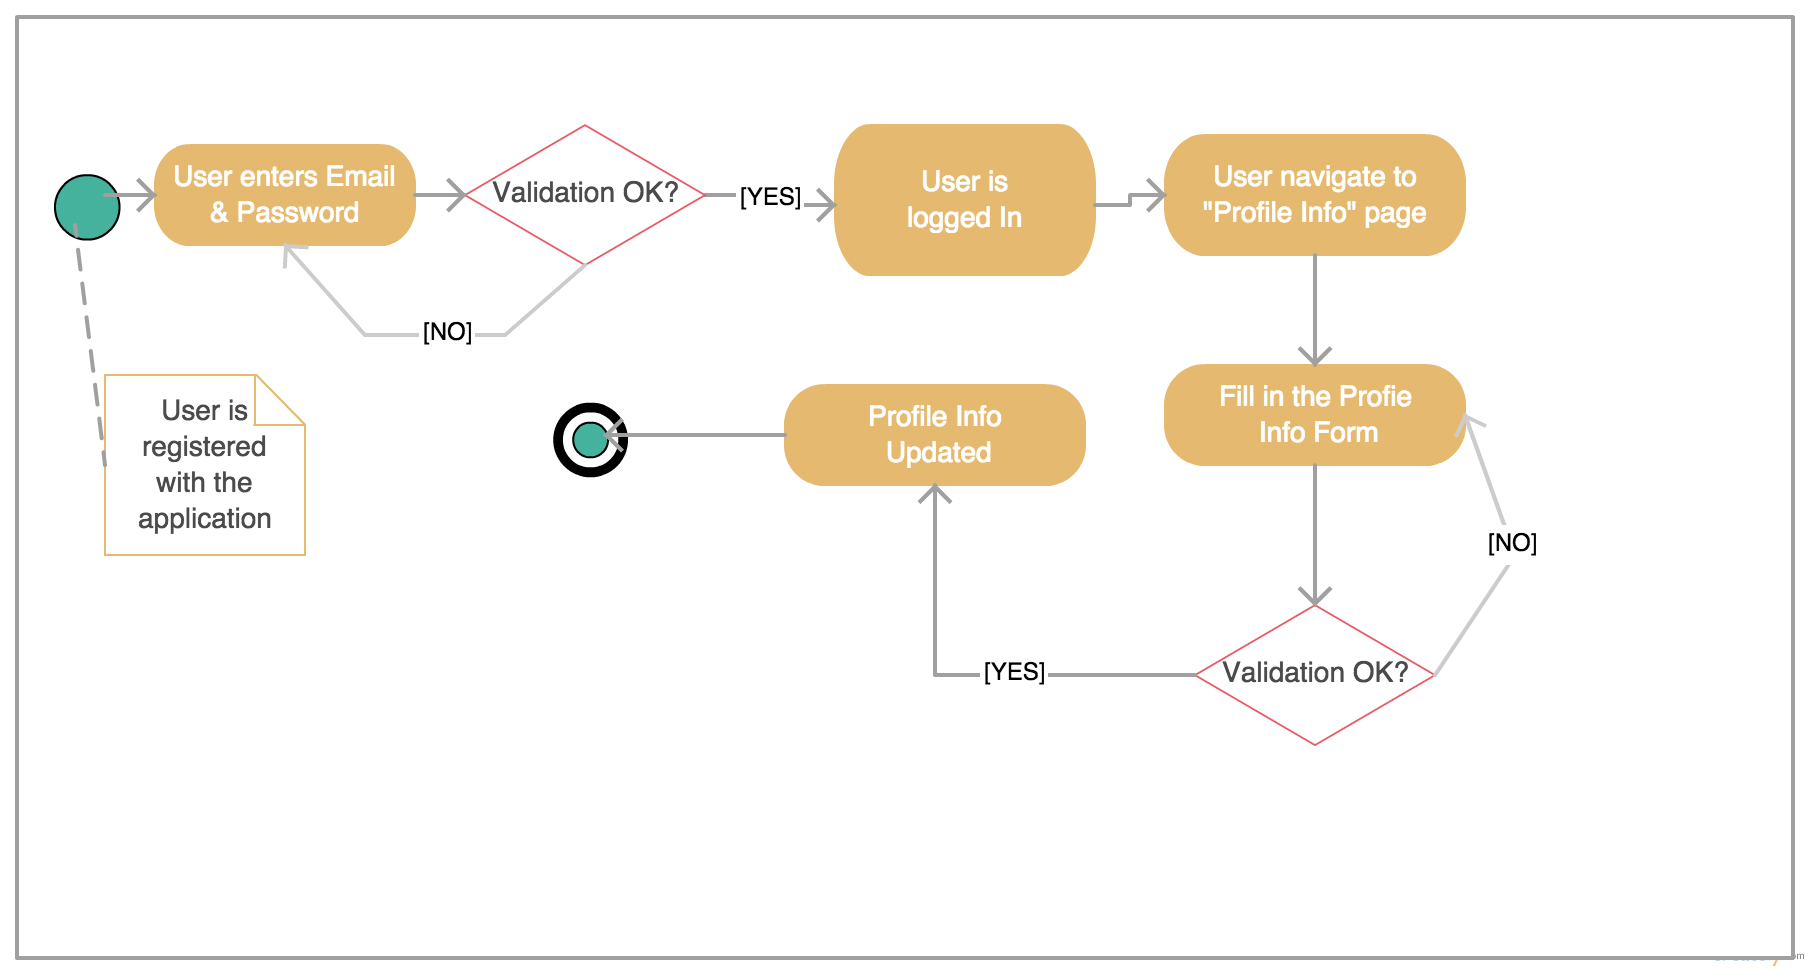
\includegraphics[width=.90\textwidth]{design/images/ad_2.jpg}
		\caption{Edit User Details activity diagram.} \label{fig:using:activitydiagram2}
	\end{center}
\end{figure}

\begin{figure}[H]
	\begin{center}
		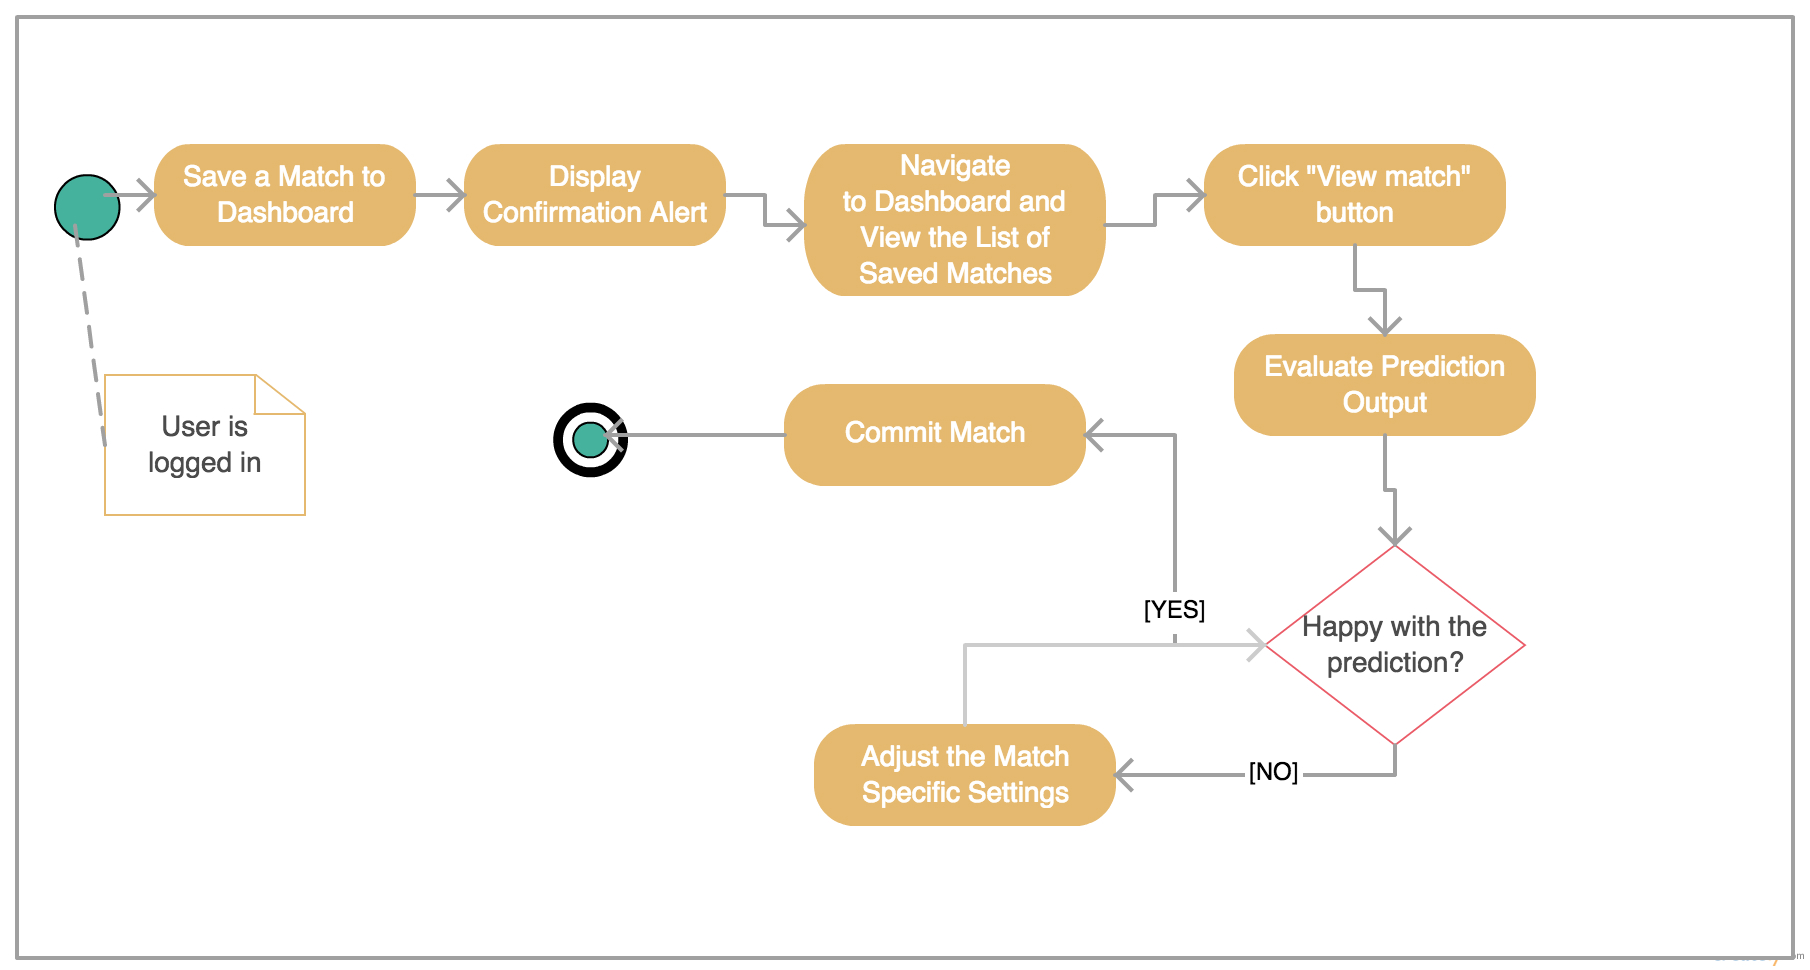
\includegraphics[width=.90\textwidth]{design/images/ad_3.jpg}
		\caption{Bet on Match activity diagram.} \label{fig:using:activitydiagram3}
	\end{center}
\end{figure}

\section{Database Schema}
\label{databaseschema_design}
The application requires a database. The data to be stored there will be represented by a set of database models. The schema for this project was developed in an iterative way along with the development of the high level features of the application - the tables and relationships between them were added gradually. The final, merged version of the diagram is a result of numerous iterations and can be found below.

\begin{figure}[H]
	\begin{center}
		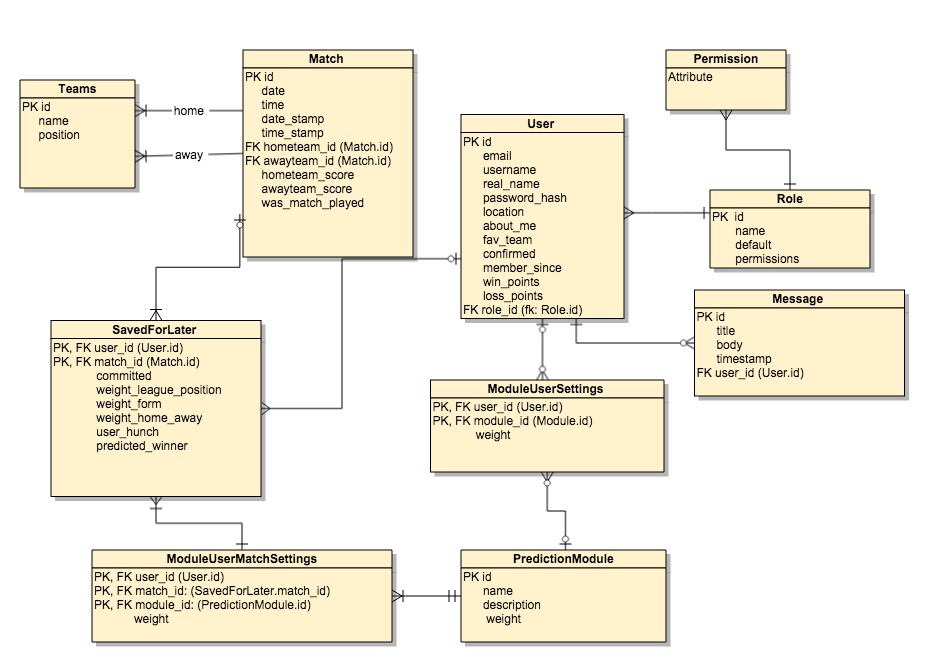
\includegraphics[width=.90\textwidth]{design/images/database_export.jpg}
		\caption{A final diagram representing tables in the database.}
		\label{fig:using:databaseschema}
	\end{center}
\end{figure}